\documentclass[12pt]{article}
\usepackage{geometry}                % See geometry.pdf to learn the layout options. There are lots.
\geometry{letterpaper}                   % ... or a4paper or a5paper or ... 
%\geometry{landscape}                % Activate for for rotated page geometry
\usepackage[parfill]{parskip}    % Activate to begin paragraphs with an empty line rather than an indent
\usepackage{./styles/daves,fancyhdr,natbib,graphicx,dcolumn,amsmath,lastpage,url}
\usepackage{amsmath,amssymb,epstopdf,longtable}
\usepackage[final]{pdfpages}
\DeclareGraphicsRule{.tif}{png}{.png}{`convert #1 `dirname #1`/`basename #1 .tif`.png}
\pagestyle{fancy}
\lhead{CE 5362 -- Surface WaterModeling}
\rhead{SPRING 2020}
\lfoot{}
\cfoot{}
\rfoot{Page \thepage\ of \pageref{LastPage}}
\renewcommand\headrulewidth{0pt}



\begin{document}
\begin{center}
{\textbf{{ CE 5362 Surface Water Modeling} \\ {Project 5}}}
\end{center}

\section*{{Introduction and Purpose}}
SToRM is a component of the USGS Multi-Dimensional Surface Water Modeling System \citep{mdswms2012}
SToRM is one of a generation of recently available 2--D hydrodynamic models available without charge or for low cost. 
In the next several exercises you will apply SToRM to several test situations where actual measurements are available in part to test the tool itself at physical scales that differ by about an order of magnitude, and to develop the skill set necessary to use the tool for an arbitrary situation.

\section*{{Problem Statement}}

\begin{enumerate}
\item Replicate the Green River example presented in class.  
As output produce a vector plot of the velocity field  and a streamline plot.
The purpose is to convince yourself you can operate the software.

\item Simulate a rectangular channel (research flume) as depicted in Figure \ref{fig:ResearchFlumePlain},
The flume elevation information is contained in the file \url{rf-plain.tpo}.  

\begin{figure}[h!] %  figure placement: here, top, bottom, or page
   \centering
   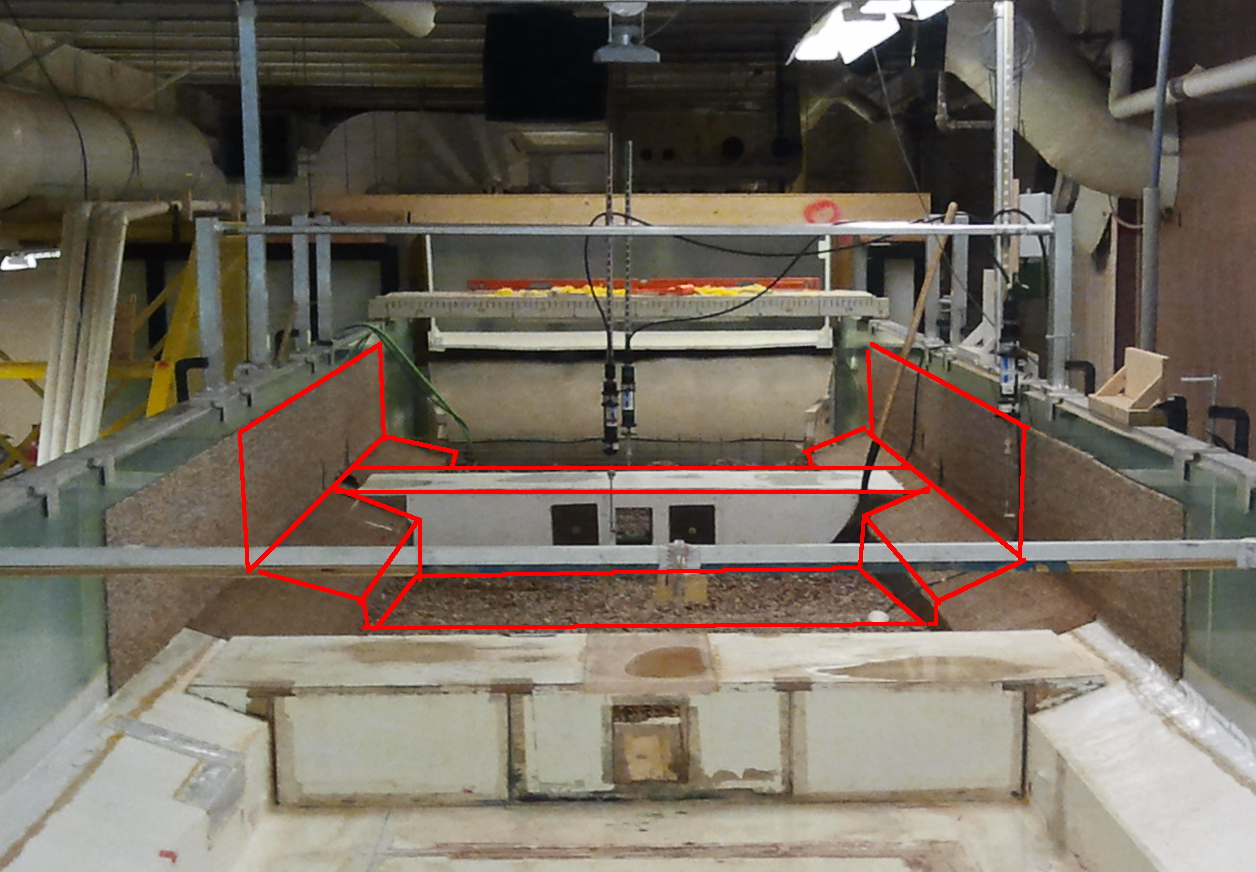
\includegraphics[width=4in]{researchflume.jpg} 
   \caption{Research flume looking upstream.  Red outline is approximate geometry of model application.  Ignore the culvert models, assume flume is a simple rectangle}
   \label{fig:ResearchFlumePlain}
\end{figure}

   Use the  following additional values to parameterize the model
\begin{itemize}
\item Initial flow depth $h = 0.30 ~ m$
\item Upstream inflow boundary condition $Q= 0.1~\frac{m^3}{s}$
\item Downstream outflow boundary condition, $H = 0.3~m$
\item Initial X-component of velocity, $U = 0.2~m/s$
\item Initial Y-component of velocity, $V = 0.0~m/s$
\item Manning's roughness coefficient $n= 0.04$
\end{itemize}

Produce simulation outputs that show the velocity distribution (vector plots), and the streamline plot, similar to Figure \ref{fig:RecterVector} and Figure \ref{fig:RecterStream}.
Discuss any steps you had to take to reflect the geometry correctly for the numerical model to function correctly.

\begin{figure}[h!] %  figure placement: here, top, bottom, or page
   \centering
   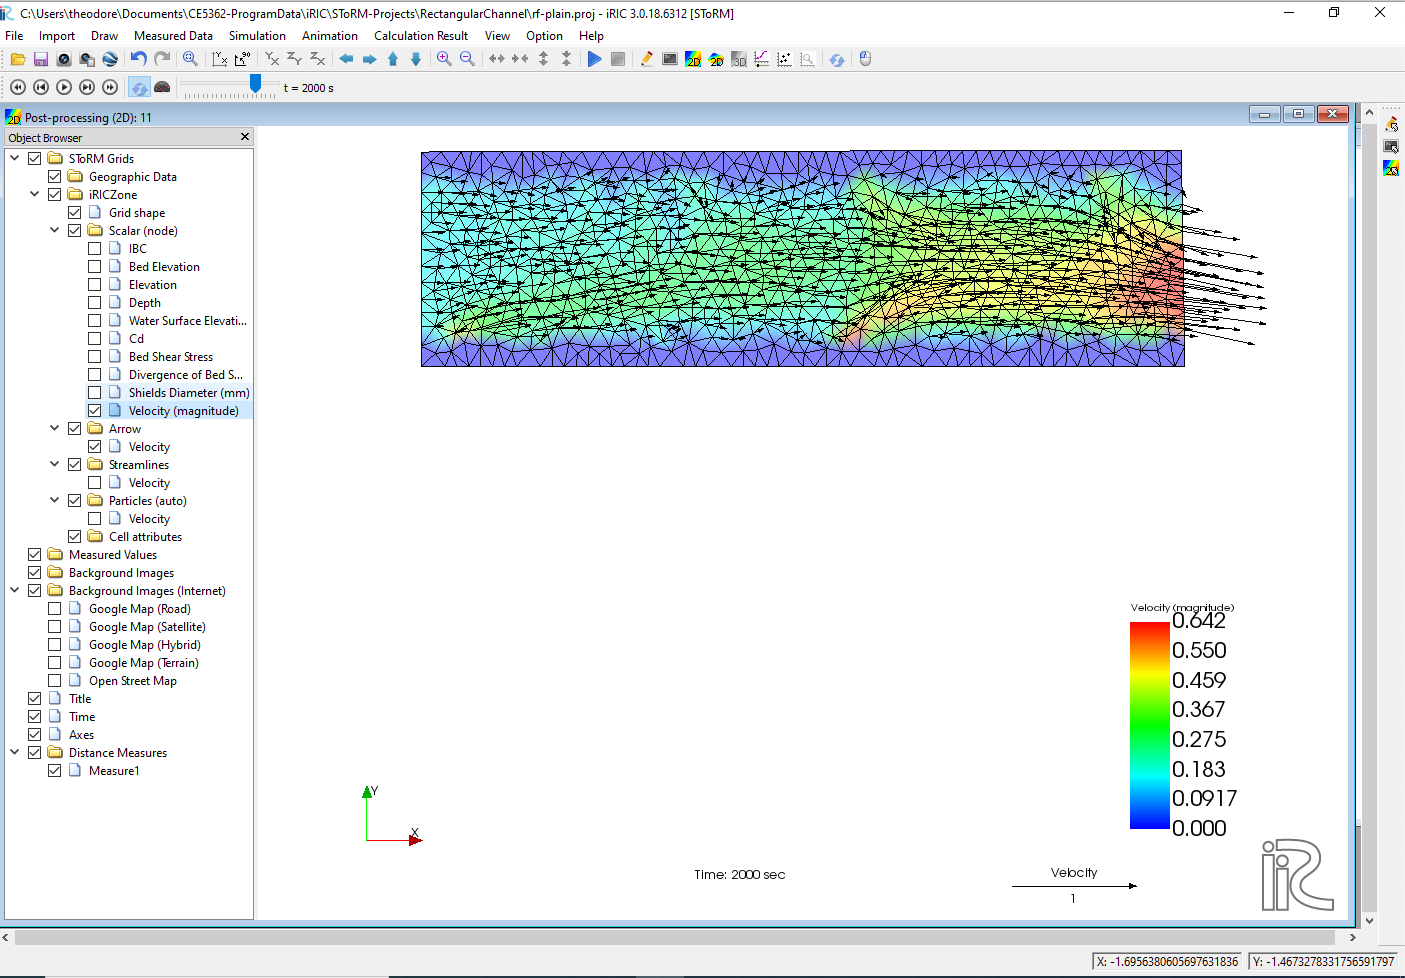
\includegraphics[height=2in]{RecterVector.png} 
   \caption{Vector plot at simulation time $t=2000~sec$, research flume, no obstruction}
   \label{fig:RecterVector}
\end{figure}

\begin{figure}[h!] %  figure placement: here, top, bottom, or page
   \centering
   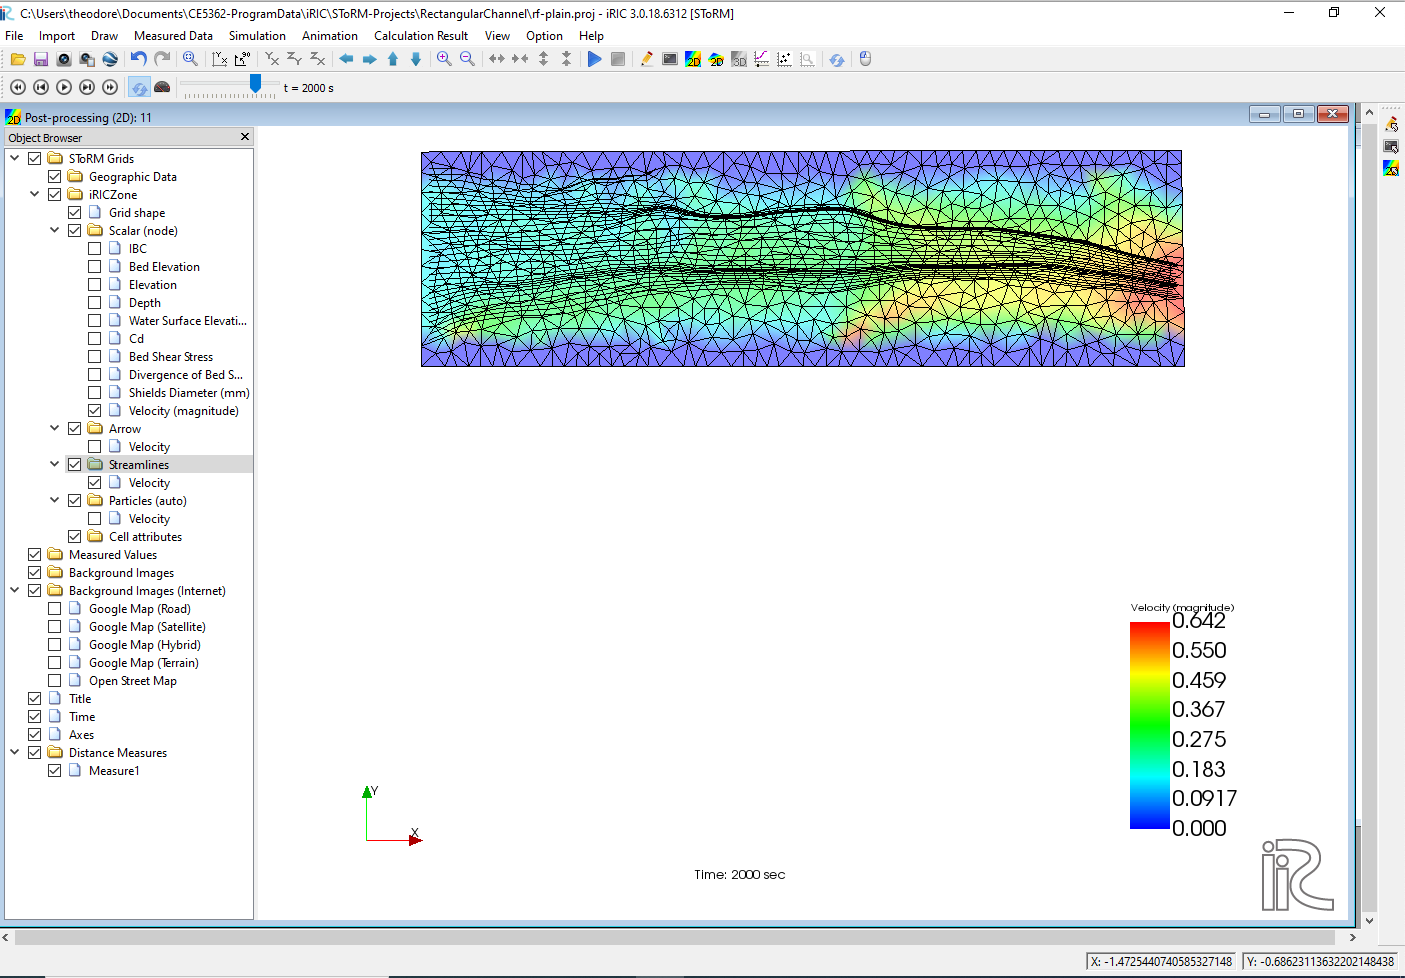
\includegraphics[height=2in]{RecterStream.png} 
   \caption{Streamline plot at simulation time $t=2000~sec$, research flume, no obstruction}
   \label{fig:RecterStream}
\end{figure}

\clearpage
\item Simulate a rectangular channel (research flume) as depicted in Figure \ref{fig:ResearchFlumeStep}, which includes the step with a cut in the middle to represent the small culverts

The flume elevation information is contained in the file \url{rf-cutstep.tpo}.  

\begin{figure}[h!] %  figure placement: here, top, bottom, or page
   \centering
   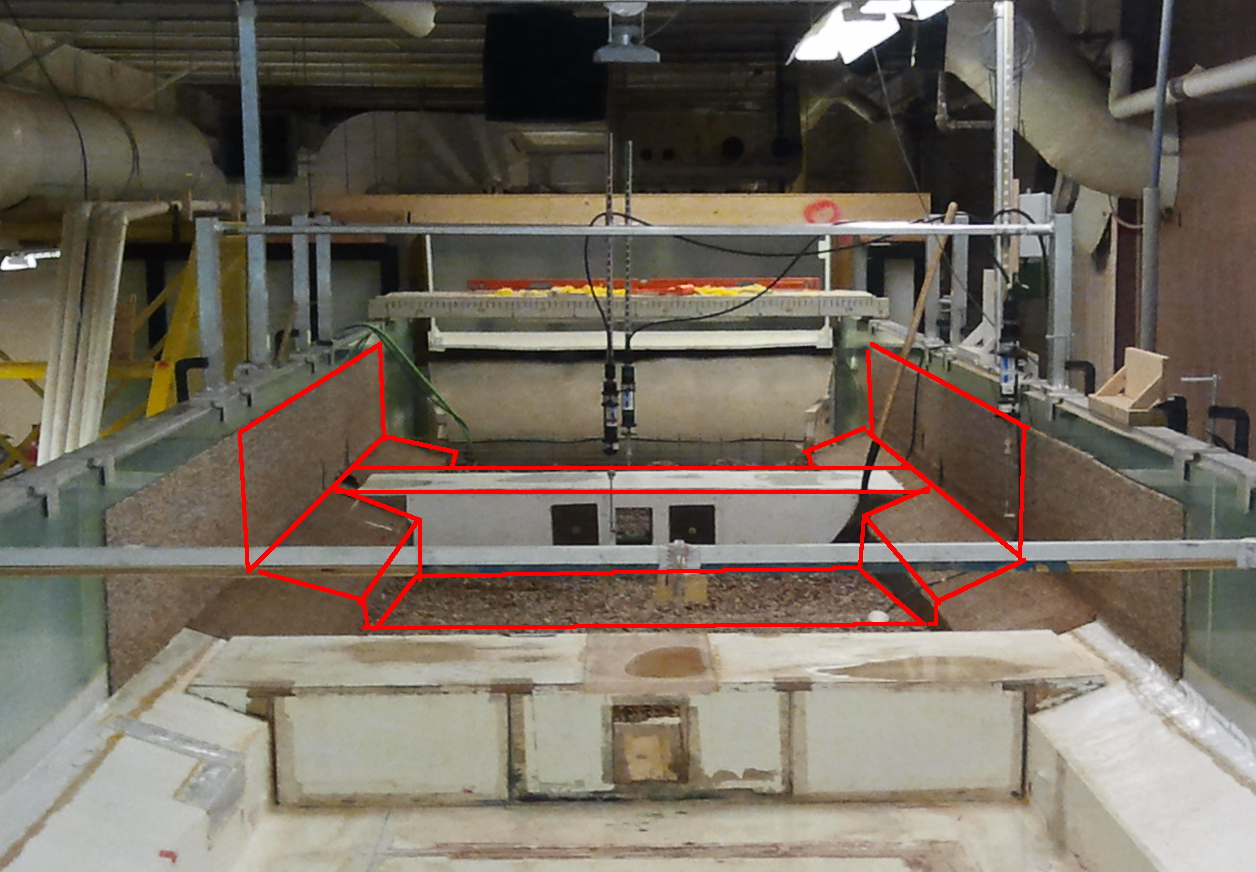
\includegraphics[width=4in]{researchflume.jpg} 
   \caption{Research flume looking upstream.  Red outline is approximate geometry of model application.}
   \label{fig:ResearchFlumeStep}
\end{figure}

   Use the  following additional values to parameterize the model
\begin{itemize}
\item Initial flow depth $h = 0.30 ~ m$
\item Upstream inflow boundary condition $Q= 0.1~\frac{m^3}{s}$
\item Downstream outflow boundary condition, $H = 0.3~m$
\item Initial X-component of velocity, $U = 0.2~m/s$
\item Initial Y-component of velocity, $V = 0.0~m/s$
\item Manning's roughness coefficient $n= 0.04$
\end{itemize}

Produce simulation outputs that show the velocity distribution (vector plots), and the streamline plot.
Discuss any steps you had to take to reflect the geometry correctly for the numerical model to function correctly.

Compare the results to the previous model, is the effect of the step apparent in the velocity or streamline diagram?



\begin{figure}[h!] %  figure placement: here, top, bottom, or page
   \centering
   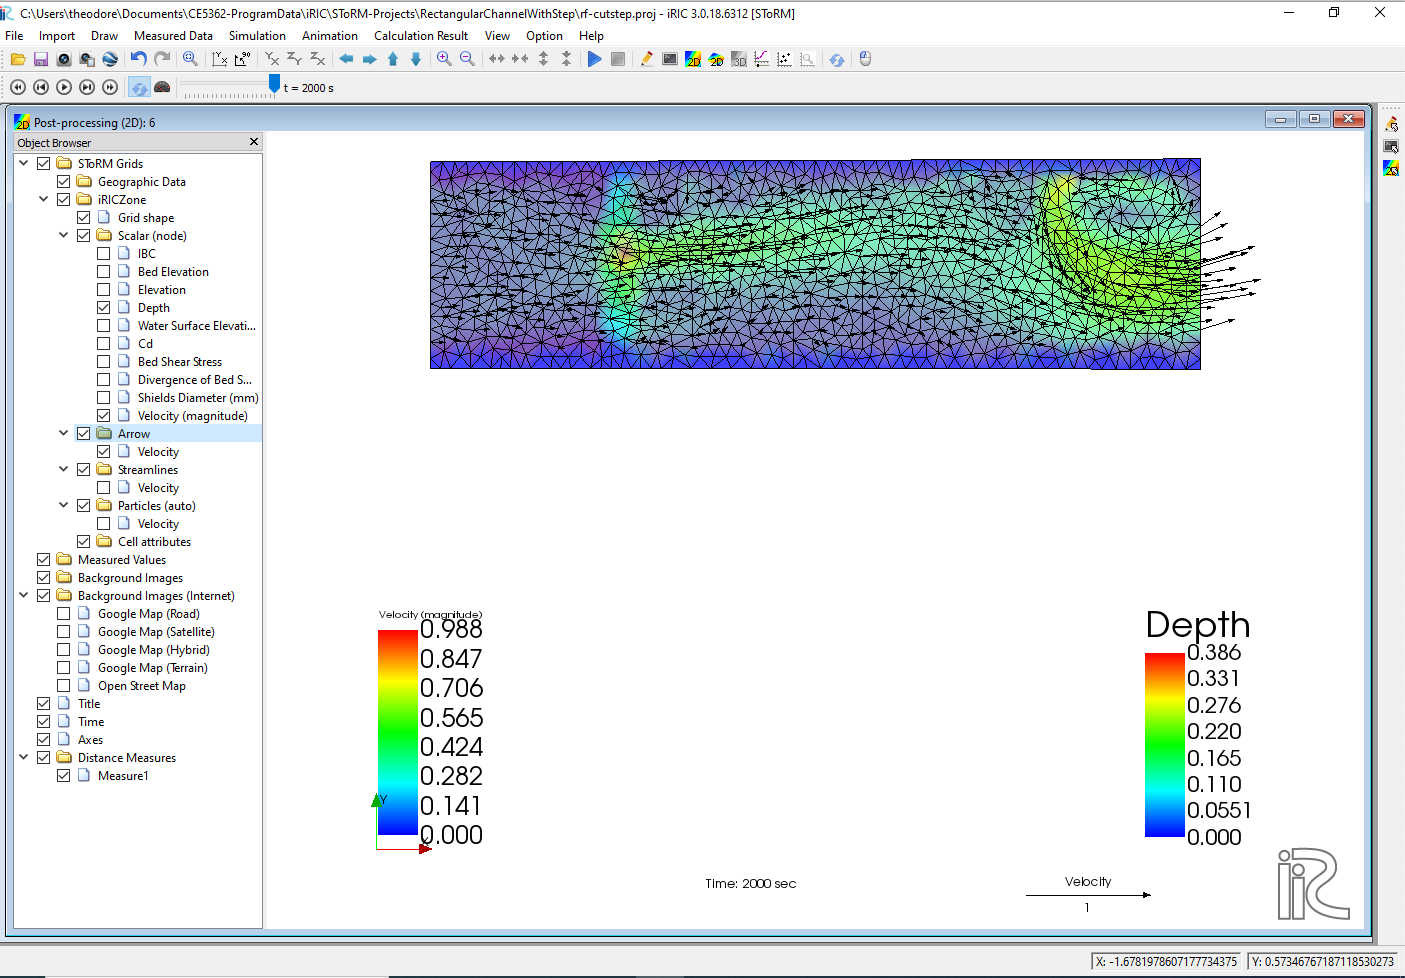
\includegraphics[height=2in]{RecterVectorStep.png} 
   \caption{Vector plot at simulation time $t=2000~sec$, research flume, with obstruction}
   \label{fig:RecterVectorStep}
\end{figure}

\begin{figure}[h!] %  figure placement: here, top, bottom, or page
   \centering
   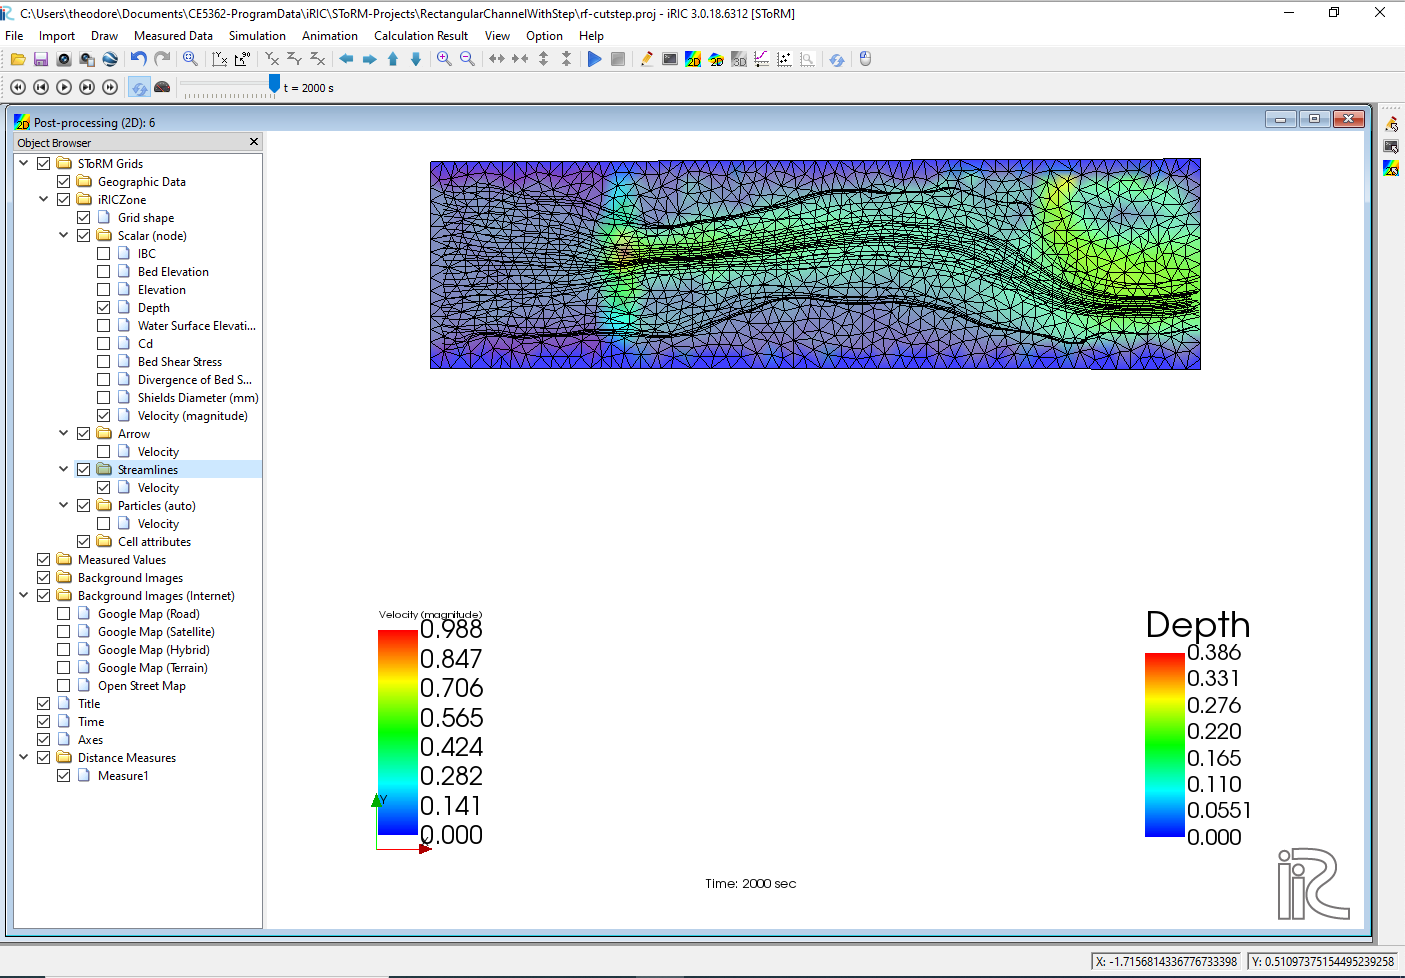
\includegraphics[height=2in]{RecterStreamStep.png} 
   \caption{Streamline plot at simulation time $t=2000~sec$, research flume, with obstruction}
   \label{fig:RecterStreamStep}
\end{figure}
\newpage

\item (Advanced) Edit the \url{.tpo} file to move the cut to one side of the flume.  Does this change the velocity pattern.  Produce output plots.
\end{enumerate}


\begin{thebibliography}{}

\bibitem[USGS, 2011]{storm2011}
{USGS Geomorphology Laboratory} (2011).
\newblock System for Transport and River Modeling.   
\url{http://wwwbrr.cr.usgs.gov/projects/GEOMORPH_Lab/project-SToRM.html} Webpage last accessed, 12 Jan 2012.

\bibitem[McDonald and others, 2012]{mdswms2012}
{McDonald, R.R., Nelson, J.M., and Bennett, J.P.}, (2012).  
\textsl{in press}. Multi-dimensional surface-water modeling system user's guide: U.S. Geological Survey Techniques and Methods, 6-B2, 136 p.

%\bibitem[Google Earth, 2011]{GoogleEarth2011}
%{Google Earth, Google Inc.}, (2011). 
%\url{http://www.google.com/earth/index.html} 
%1600 Amphitheatre Parkway Mountain View, CA, 94043
%
%\bibitem[Golden Software, 2010]{surfer2010}
%{Golden Software, Inc.}, (2010). Surfer 10.
%809 14th Street, Golden, Colorado 80401-1866, U.S.A.
%Phone: 303-279-1021 Fax: 303-279-0909
%\url{www.GoldenSoftware.com}

%\bibitem[Dixon, J. 2011]{dixon2011}
%{Dixon, J.}, (2011). 
%A Relation Between Select Hydraulic Properties and Sediment
%Transport Volume Through Experimental Culvert Configurations
%and Techniques for Measuring Sediment Transport Volumes.
%MS Thesis, Department of Civil and Environmental Engineering, Texas Tech University, 117 p.

\end{thebibliography}

\end{document}